\documentclass[UTF-8]{ctexart}

\usepackage{amsmath}
\usepackage{graphicx}
\usepackage[a4paper]{geometry}
\usepackage{cleveref}
\usepackage{gbt7714}
%opening
\usepackage{listings}
\usepackage{color}
\usepackage{colortbl}
\usepackage{xcolor}
\usepackage{array}
\usepackage{enumerate}
\usepackage{listings}
\definecolor{dkgreen}{rgb}{0,0.6,0}
\definecolor{gray}{rgb}{0.5,0.5,0.5}
\definecolor{mauve}{rgb}{0.58,0,0.82}


\lstset{frame=tb,
	language=Python,
	aboveskip=3mm,
	belowskip=3mm,
	showstringspaces=false,
	columns=flexible,
	basicstyle={\small\ttfamily},
	numbers=none,
	numberstyle=\tiny\color{gray},
	keywordstyle=\color{blue},
	commentstyle=\color{dkgreen},
	stringstyle=\color{mauve},
	breaklines=true,
	breakatwhitespace=true,
	tabsize=3
}

\title{密码分析学-第四次作业}
\author{第八组}

\begin{document}


\maketitle
\begin{abstract}
	对于四轮的高偏差线性壳寻找,我们使用了树的数据结构,通过中间相遇的思想,以线性壳头部和尾部为根节点分别建立前向树和后向树,在中间第二轮进行寻找碰撞,同时在树的每一个结点使用一个数字存储从根节点到此节点路径上的偏差值,最后使用堆积引理进行求解整体路径偏差值,并对满足头部和尾部的掩码的路线概率进行求和,寻找取绝对值后的高概率线性壳.\par
	\setlength{\parindent}{2em} 基于寻找到的高偏差线性壳以及选择的明密文对数,我们进行线性分析,每个线性壳可以构造一个区分器。其中按照输出掩码所涉及到的S盒,我们将其分成了四类,分别为:输出中第一个S盒活跃、第二个S盒活跃、第三个S盒活跃,第四个S盒活跃;可分别用来恢复第五轮CipherFour的4个bits的密钥,对四种S盒对应密钥的线性壳进行筛选,选择出偏差大于0.02以及最大偏差明显大于其他位置的线性壳,对此部分线性壳进行对选择的明密文对进行二次计数,选择二次计数器中计数数值最大的数作为最终猜测的密钥。\par
\end{abstract}
\newpage


\tableofcontents
\newpage

\section{线性分析}
主要有两种思路,4+1和1+3+1,我们选择了4+1模式,即四轮线性壳,一轮恢复密钥.至于为什么不选择1+3+1,在结果分析中给出了原因.
\subsection{分析思路}
\subsubsection{寻找线性壳}
\paragraph{算法思路}
\begin{enumerate}
	\item 首先需要生成LAT表,对于给定S盒,利用如下伪代码\cref{fig:latgen}进行遍历,得到输入掩码输出掩码对应的偏差,如图\cref{fig:lat}.
	\begin{figure}[!htbp]
		\centering
		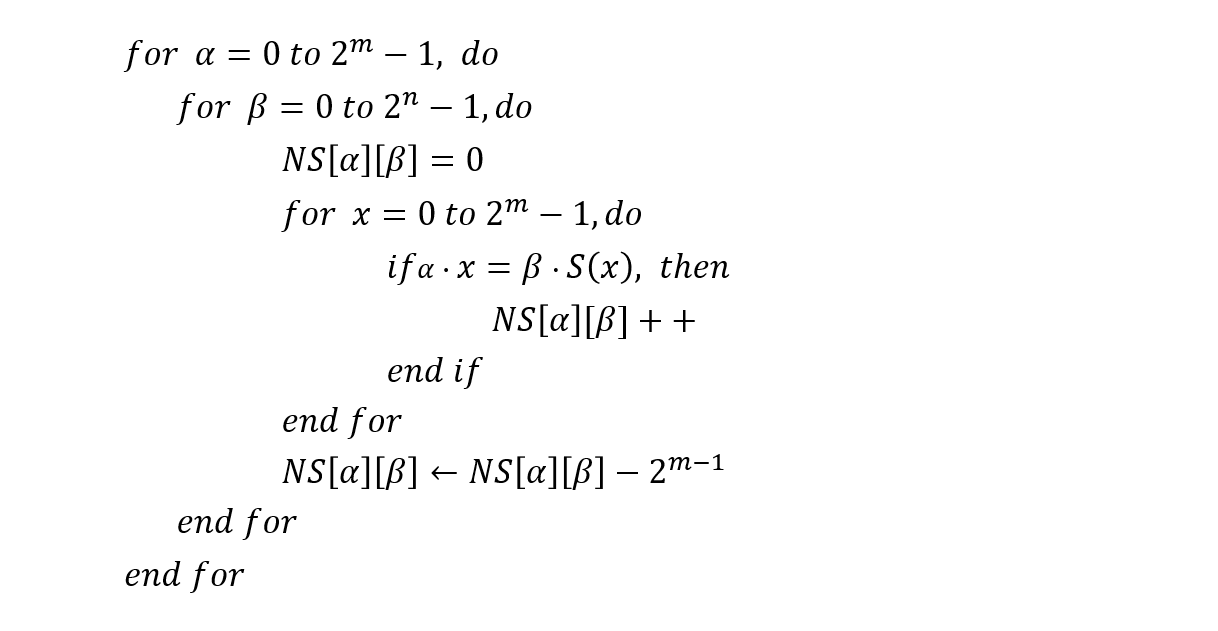
\includegraphics[width=0.7\linewidth]{LAT_gen}
		\caption{LAT生成算法}
		\label{fig:latgen}
	\end{figure}
	\begin{figure}[!htbp]
		\centering
		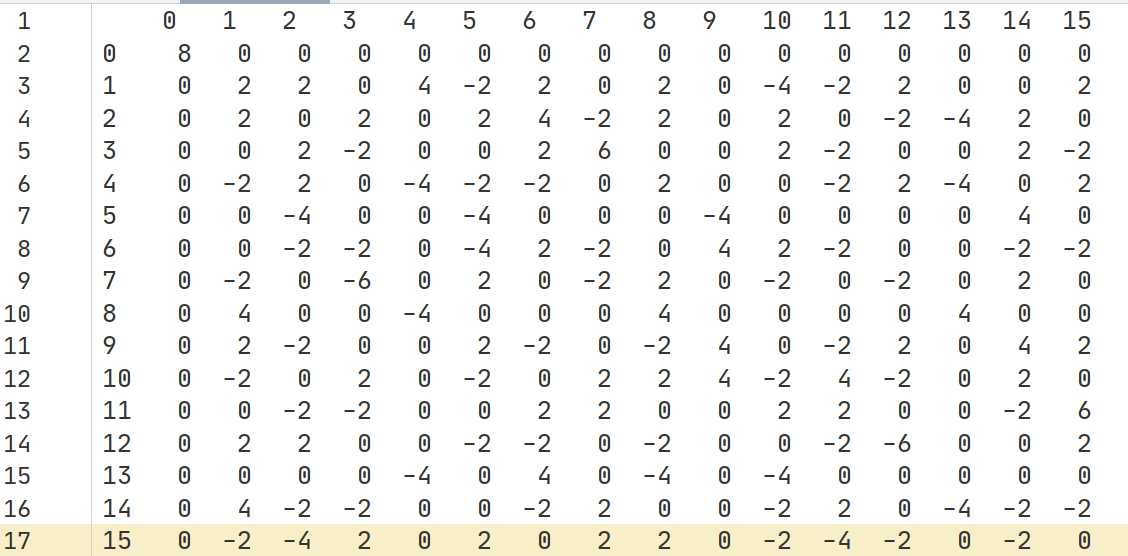
\includegraphics[width=0.7\linewidth]{LAT}
		\caption{LAT表}
		\label{fig:lat}
	\end{figure}
	
	
	
	\item 根据堆积引理要求,我们发现对于高偏差线性壳头部与尾部掩码应该尽可能的多0,所有我们进行寻找16bit掩码中1的个数等于1的线性壳,同时需要满足每一轮的线性逼近式只含有1个活跃S盒(输出掩码非零)。
	\item 遍历第一部得到的筛选后的线性壳头部与尾部.对输入掩码(线性壳头部)进行如下操作:
	\begin{enumerate}
		\item 以输入掩码为多叉树根结点,以此掩码为结点Tag,同时存储偏差数组[],同时对每一轮设置一个栈,初始为空,将继续进行下一轮的结点ID值入栈.此时为根节点入栈
		\item 对上一轮栈中每一个结点出栈,以此为节点,根据LAT表进行得到对应的可能的输出掩码,对每一个可能的输出掩码进行P置换,得到一轮过后的输出掩码,同时进行将对应的输出值进行堆积引理计算,对结果取绝对值后进行阈值(设置为1/128)比较,如果小于阈值,则对此节点不再进行第二轮的寻找,大于或等于,则入栈,进行下一轮操作
		\item 对入栈的数据进行出栈操作,继续进行第2步的操作,最终得到一个前向的多叉树.
	\end{enumerate}
输出掩码(线性壳尾部)进行如下操作:
\begin{enumerate}
	\item 以输出掩码为多叉树根结点,以此掩码为结点Tag,同时存储偏差数组[],同时对每一轮设置一个栈,初始为空,将继续进行下一轮的结点ID值入栈.此时为根节点入栈
	\item 对上一轮栈中每一个结点出栈,以此为节点,首先进行P置换,根据LAT表进行得到对应的可能的输入掩码,同时存储对应的偏差值,得到一轮过后的掩码,同时进行将对应的输出值进行堆积引理计算,对结果取绝对值后进行阈值(设置为1/128)比较,如果小于阈值,则对此节点不再进行第二轮的寻找,大于或等于,则入栈,进行下一轮操作
	\item 对上一轮入栈的数据进行出栈操作,继续进行第2步的操作,最终得到一个后向的多叉树.
\end{enumerate}
	\item 对两个树进行如下处理:
	\begin{enumerate}
		\item 筛选出到达第三轮的路径,并对叶节点的ID与Tag(掩码值)进行取出处理
		\item 对两个树取出的Tag进行碰撞,如果相等,则说明此结点(Tag)对应
	一条路线,利用Tag对应的ID将两个结点存储的偏差数组合,利用堆积引理计算对应的偏差值
		\item 对所有发生碰撞的四轮路径的偏差值进行求和(带正负号)并存储
	\end{enumerate}
	\item 换输入掩码,输出掩码进行重复以上操作
\end{enumerate}

对于四轮的高偏差线性壳寻找,我们使用了树的数据结构,通过中间相遇的思想,以线性壳头部和尾部为根节点分别建立前向树和后向树,在中间第二轮进行寻找碰撞,同时在树的每一个结点使用一个数字存储从根节点到此节点路径上的偏差值,最后使用堆积引理进行求解整体路径偏差值,并对满足头部和尾部的掩码的路线概率进行求和,寻找取绝对值后的高概率线性壳.




\subsection{运行结果与程序效率测试}
\paragraph{阈值选取}
我们发现,如果一个线性壳不设置阈值,则会有很大可能出现路线爆炸,运行时间也会减慢,所以可以通过设置阈值来实现最终线性壳的寻找,具体测试与结果如下\cref{fig:yuzhi}
	\begin{figure}[!htbp]
	\centering
	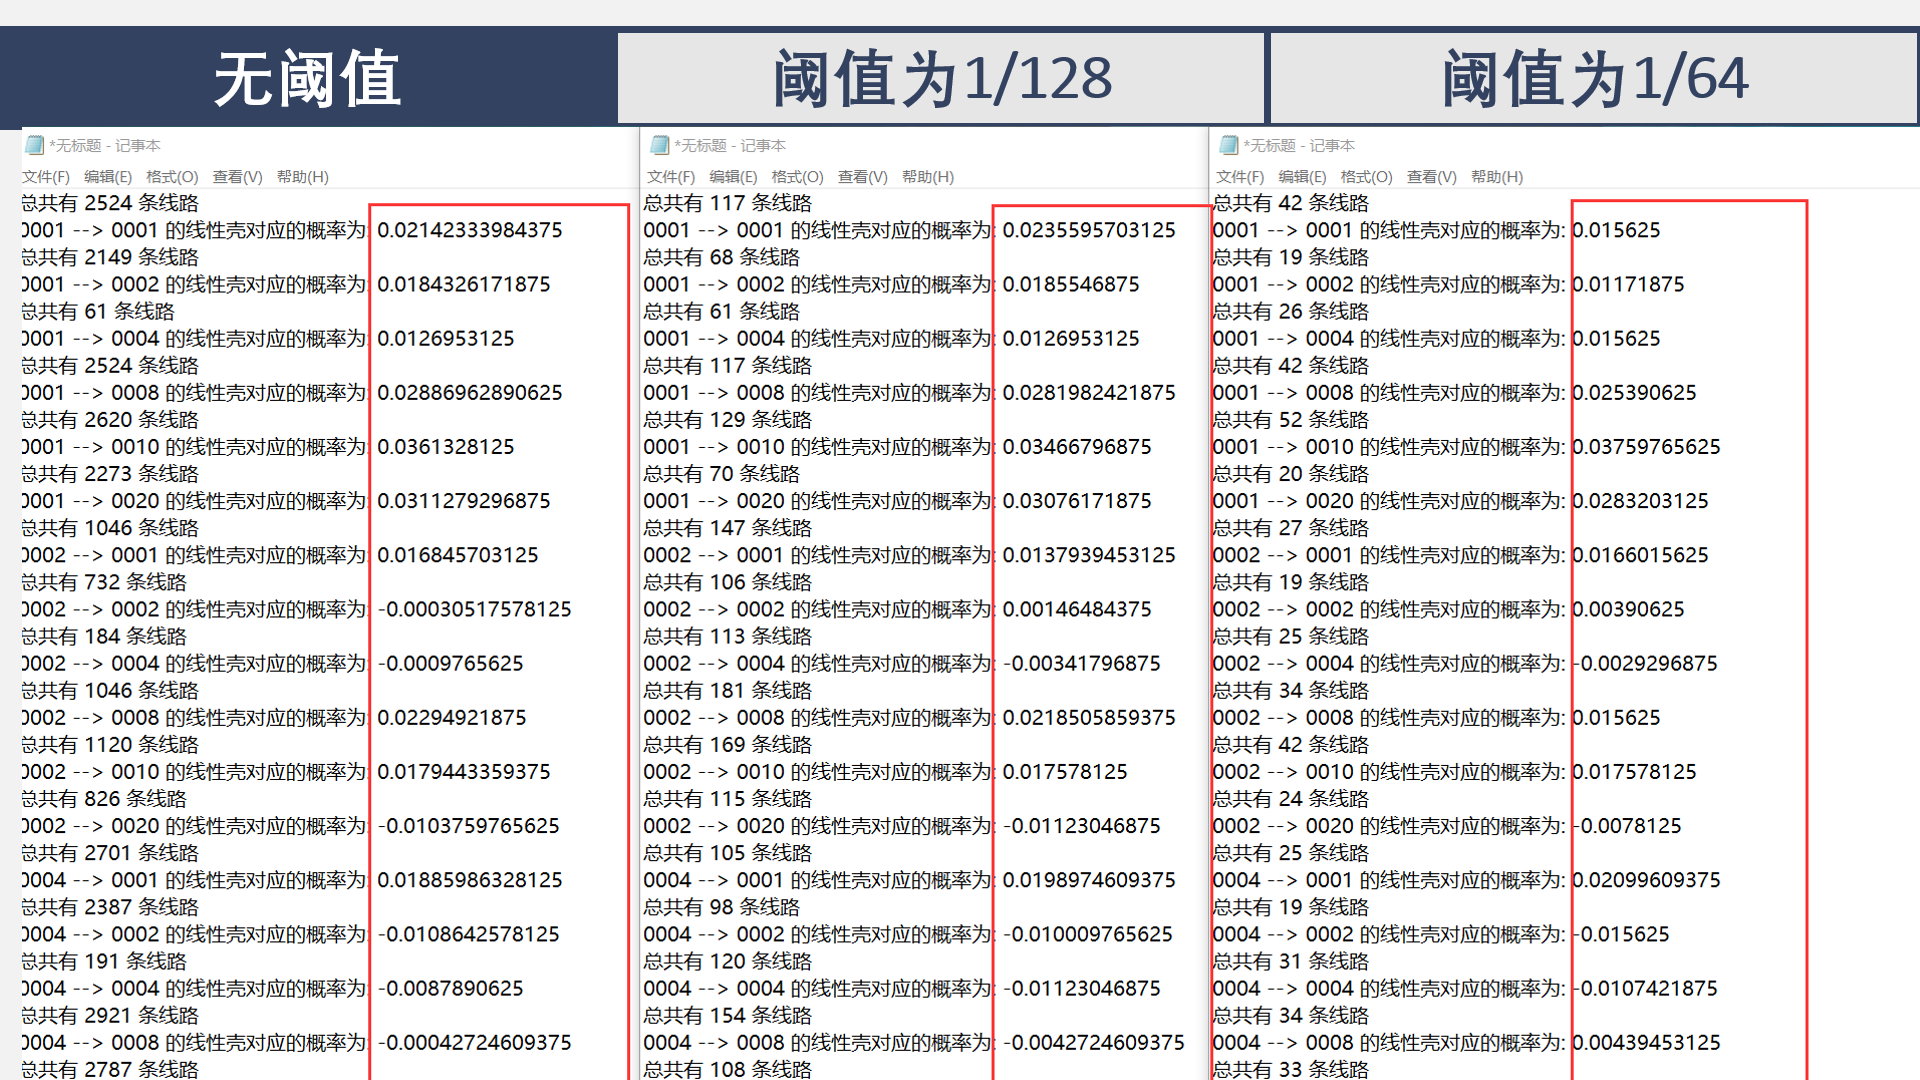
\includegraphics[width=0.7\linewidth]{yuzhi}
	\caption{设置阈值与否的结果对比}
	\label{fig:yuzhi}
\end{figure}
速度测试结果如下\cref{fig:yuzhit}
\begin{figure}[!htbp]
	\centering
	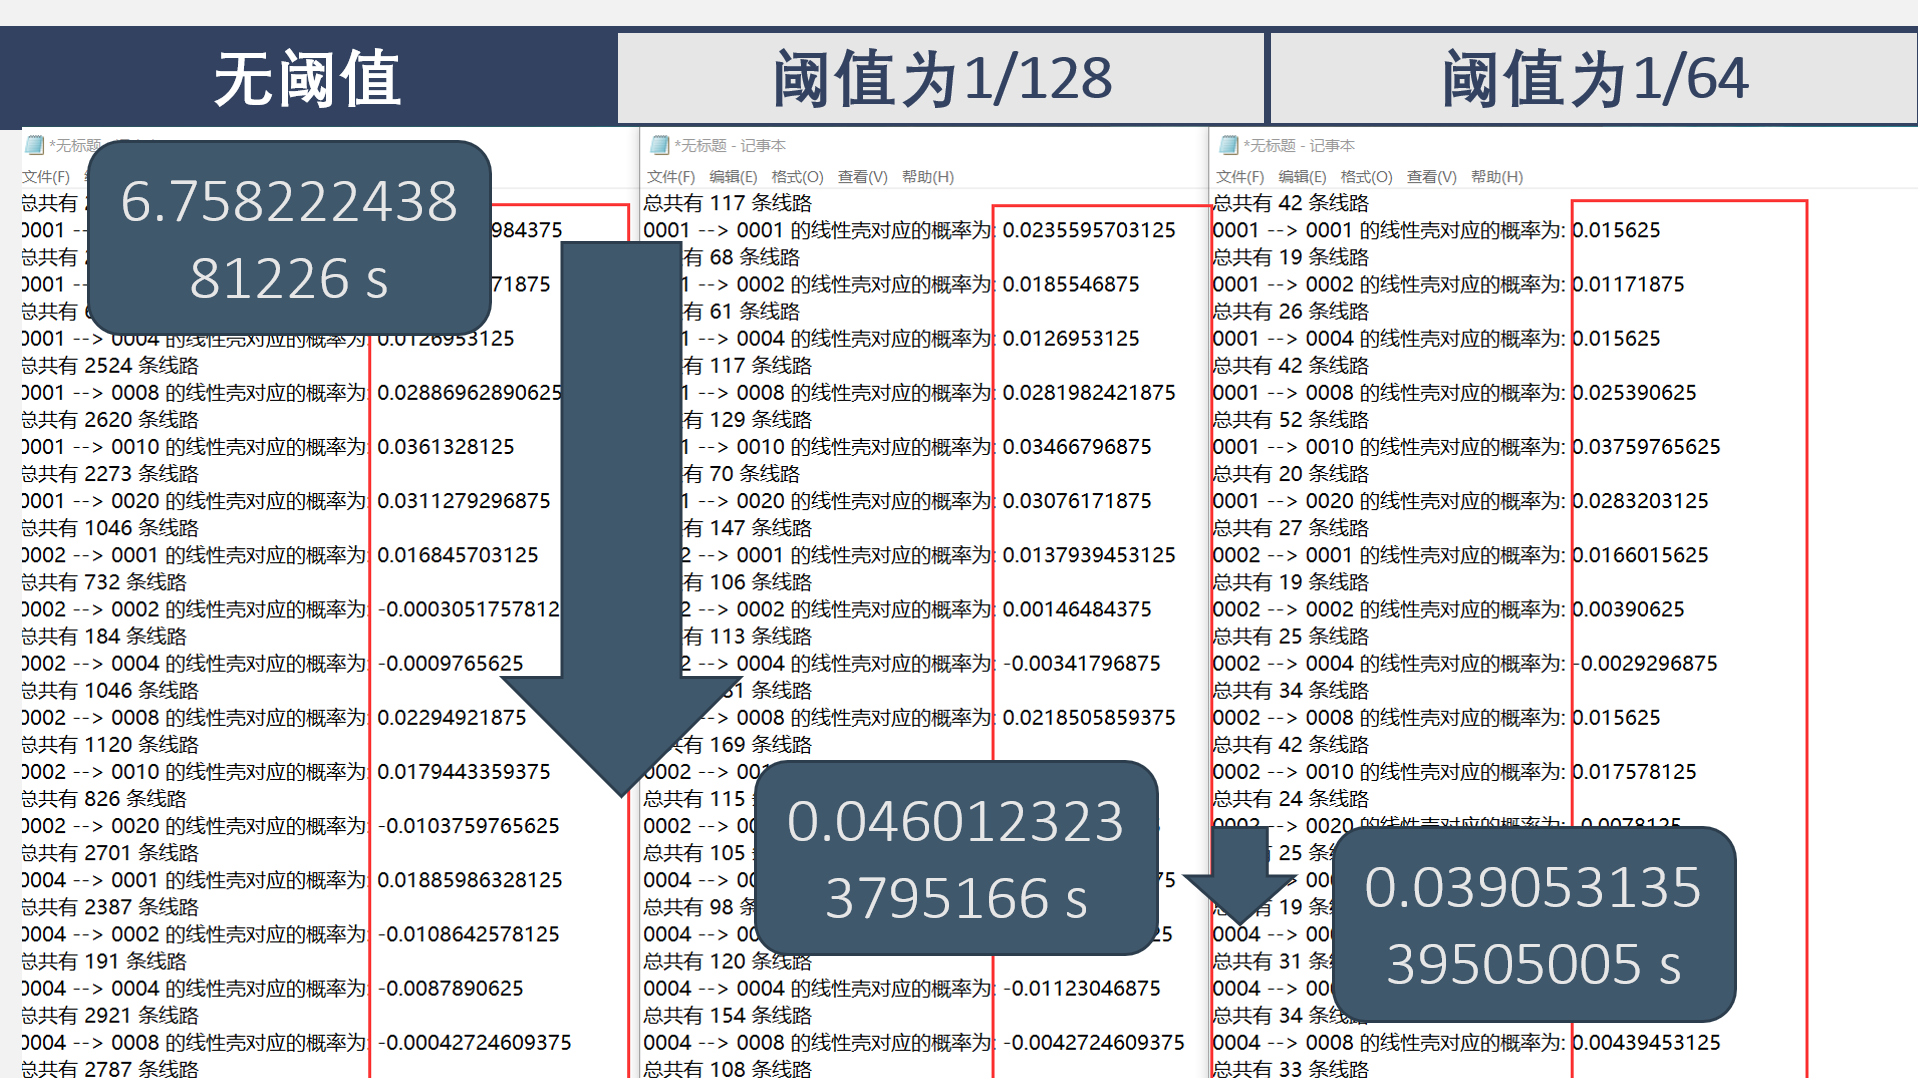
\includegraphics[width=0.7\linewidth]{yuzhi_time}
	\caption{设置阈值与否的速度对比}
	\label{fig:yuzhit}
\end{figure}
根据速度与结果准确度分析,我们最终选择阈值为$\frac{1}{128}$,进行测试256组线性壳得到对应偏差值.

\paragraph{运行结果}

运行附件中$Linear_kernel.py$程序中的FindLinearHull类中的MainFunction方法,参数中传入对应输入掩码与输出掩码对,可以输出寻找到的线路以及对应的偏差值,同时,为了可视化数据与分析数据,我们对前向树与后向树进行可视化输出,对所有树进行存储,具体文件见附件$treeForward.txt$和$treeBackward.txt$,以输入掩码为'8000',输出掩码为'0008'举例,对应阈值为1/128时,可以得到20条掩码路线,求和后得到的偏差概率0.044921875,其中前向树部分图\cref{fig:F},后向树部分图见\cref{fig:B}
	\begin{figure}[!htbp]
	\centering
	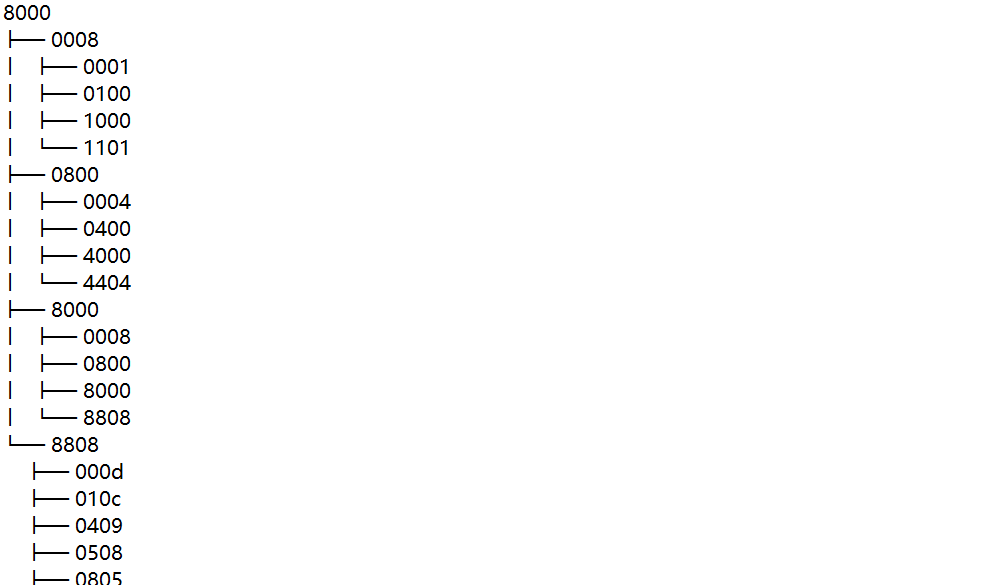
\includegraphics[width=0.7\linewidth]{treeF}
	\caption{输入掩码为'8000'时前向树部分结构图}
	\label{fig:F}
\end{figure}
\begin{figure}[!htbp]
	\centering
	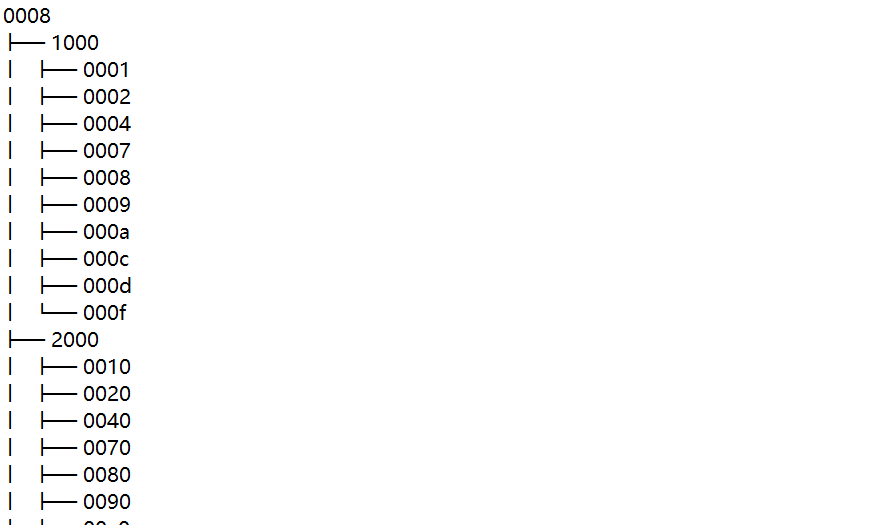
\includegraphics[width=0.7\linewidth]{treeB}
	\caption{输出掩码为'0008'时后向树部分结构图}
	\label{fig:B}
\end{figure}
为了后续进行线性分析,同时对遍历的线性壳以及对应偏差进行输出到附件$Linear$,部分结构如图\cref{fig:hull}
\begin{figure}[!htbp]
	\centering
	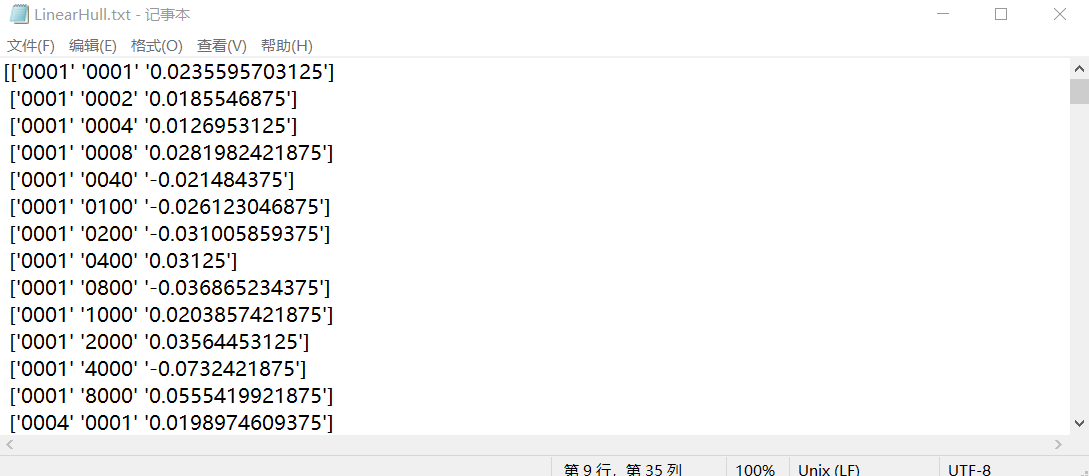
\includegraphics[width=0.7\linewidth]{Hull}
	\caption{线性壳输出文件部分数据图}
	\label{fig:hull}
\end{figure}
\paragraph{测试环境}
\begin{table}  [htbp]
	%	\Large  
	\caption{运行环境}  
	\begin{center}  
		\begin{tabular}{|l|l|l|l|l|l|l|} 
			\hline
			cpu   & 核心数 & 线程数 & 一级cache & 运行环境  \\ \hline
			IntelCore i5 826OU & 4     & 8     & 4*32KB & pycharm  \\ \hline				
		\end{tabular}  
	\end{center}  
\end{table}

\subsection{基于线性壳的线性分析}
\subsubsection{原理介绍}
不是明文和密文的取值决定了密钥取,而是密钥取值决定了线性逼近式的取值,这是由于在LAT表的构造过程中,我们是基于密钥的取值进行遍历而得到的LAT表,从而决定了明密文异或值的偏差。因为线性逼近式的存在,密钥某些比特的异或值等于中间变量的异或值,导致中间变量的异或值分布不均匀,从而可恢复外层密钥.
\subsubsection{算法介绍}

在上面寻找线性壳部分我们找到了多个四轮的线性壳及其对应的偏差,每个线性壳可以构造一个区分器。其中按照输出掩码所涉及到的S盒,我们将其分成了四类,分别为:输出中第一个S盒活跃、第二个S盒活跃、第三个S盒活跃、第四个S盒活跃;可分别用来恢复第五轮CipherFour的4个bits的密钥。根据得到的线性壳,以及对应的偏差,我们可以固定偏差值为0.03,根据老师给定参数,求出选取对应个数的明密文对$$
\begin{aligned}
&2\left|p-\frac{1}{2}\right|^{-2} \approx 2222 \uparrow \text { 明密文对 }\\
&8\left|p-\frac{1}{2}\right|^{-2} \approx 8888 \uparrow \text { 明密文对 }
\end{aligned}
$$
后续分析,都是基于这已选择的2222或者8888个明密文对
一次线性分析的流程如下:
\begin{enumerate}
	\item 根据区分器的输出确定得到中间状态需要恢复的密钥比特,假设需要恢复第一个S盒对应的4bits密钥。对每个可能的候选密钥$gk_i$,设置相应的$2^4$个计数器$T_0^{i}$,并初始化为0。
	\item 随机选取N个明文对(m,c),在这里我们将分别统计$N=2|p-1/2|^{-2}$、和$N=8|p-1/2|^{-2}$ 时的情况。
	\item 对每一个密文c,分别利用$2^{4}$个$gk_i$密钥得到第四轮输出对应的4bits中间状态Q。计算线性逼近式的左边是否为0,若成立,则给相应的计数器$T_0^{i}$加1。
	\item 将$2^4$个$gk_i$按照$|T_0^{i}-\frac{N}{2}|$的值从大到小排序,其中前$2^2$个$gk_i$作为候选的正确密钥。
\end{enumerate}
同时我们发现,有很多线性壳比如8000-->8000等并不会得到正确密钥,所以我们需要对cipherfour算法进行随机性测试,利用大数定理,测试其中8000到8000线性壳偏差数的每一个结果对应随机分布出现的概率,如图\cref{fig:gauss},我们可以得到某一个线性壳的对应测试随机性的好坏.
\begin{figure}[!htbp]
	\centering
	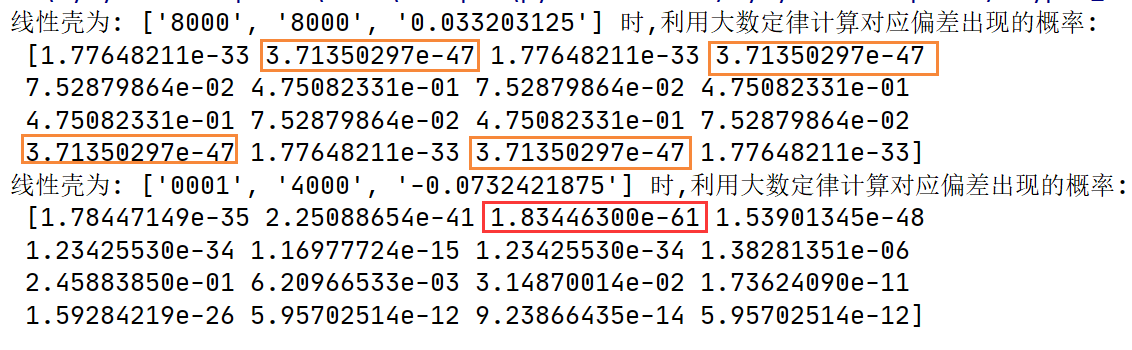
\includegraphics[width=0.8\linewidth]{Gauss}
	\caption{高斯分布表}
	\label{fig:gauss}
\end{figure}

因此,并不是所有线性壳都可以使用,所以我们会进行线性壳筛选,选择可以使用的线性壳,筛选方案如下:
\begin{enumerate}
	\item 
	偏差,选择偏差大于等于0.02的
	\item 选择计数器中最大偏差明显大于其他偏差的.(原因在上一段)
\end{enumerate}

为了提高正确率,同时充分利用已经生成的线性壳,下面,我们将进一步确定正确密钥:
 \paragraph{二次计数充分利用线性壳} 为了充分利用选择的明密文对,可以得到的多个线性壳进行分析,对每一个S盒位置对应的4bit密钥,维护一个二次计数数组,将每一个线性壳得到的一个计数器中偏差排前4位的密钥进行二次计数.
	比如:对$['0008','0010','0.05517578125']$ 分析
	此时恢复K5中第 2 个位置密钥,排名前4位的是: $[13,10,7,11]$
	对此4个位置的二次计数数组加1.
	最后取这个数组中计数最大的即为密钥位置
\subsubsection{运行结果}
经过分析,运行结果如下\cref{fig:res,fig:res2}
\begin{figure}[!htbp]
	\centering
	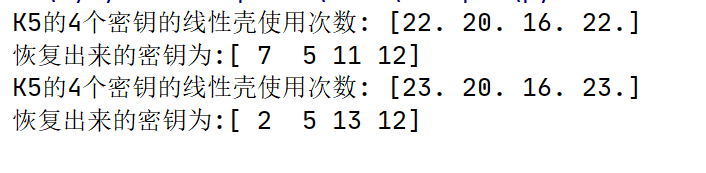
\includegraphics[width=0.8\linewidth]{Res}
	\caption{运行结果1}
	\label{fig:res}
\end{figure}

\begin{figure}[!htbp]
	\centering
	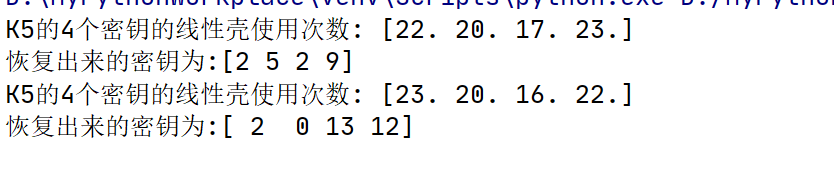
\includegraphics[width=0.8\linewidth]{Res2}
	\caption{运行结果2}
	\label{fig:res2}
\end{figure}
\paragraph{效率分析}
其中,由于明密文对均为已知,所以加密过程所耗费时间可以忽略,主要耗费时间为反向的一轮加密,由于每个线性壳需要进行16个可能的密钥一一测试,所以耗费很多时间,运行一次大约需要2分钟.
\subsubsection{结果分析}
\paragraph{结果分析} 
\begin{itemize}
	\item 为什么不用1+3+1?CipherFour加密最后一轮出现很多线性壳具有很差的随机性,如果加上第一轮,那么可以使用的线性壳就更少了
	\item 在本实验中,我们利用的线性壳均是只涉及一个活跃S盒,并且掩码非0。理论上多个S盒的高偏差线性壳可能存在,但是会耗费很多算力,所以未进行考虑.
	\item 在本算法中,我们分别选取明文数为$2|p-1/2|^{-2}|$和$8|p-1/2|^{-2}$进行线性分析,经过课上的理论分析,我们知道其成功的概率依次为:$48.6\%,96.7\%$。在上面的运行结果中,可以看到,其密钥猜测正确的概率在增大,这与理论相符。
	\item 理论上我们4+1恢复出K5所有密钥后,可以进行解密一轮,继续使用3+1恢复K4所有密钥,但是需要考虑的是注意随着轮数变少,随机性的减弱,加密的随机性会更差,可能就很难恢复出来正确密钥了
	\item 虽然低偏差的线性壳也会出现较高的成功率,但是其所需的明文数会增多,这将提高算法的复杂度。
\end{itemize}
\subsubsection{改进方向}
\begin{enumerate}
	\item 是否有输出差分涉及多个S盒的高偏差线性壳?
	\item 在二次计数时,我们可以尝试赋予不同的权重。比如最大的计数器每次加 1,第二大的加 0.8,第三大加 0.7... 提高准确率
	\item 有更好的线性壳筛选方案?\textbf{尝试过使用方差进行筛选线性壳,即对偏差计数器求方差,与删掉最大偏差后的计数器再求方差结果差值对比,如果大于设置的某个阈值,即保留,但是由于数据量等因素,导致对应选取的阈值得到分析的最终结果不太理想,所有没有再后续分析.}
	\item 3+2模式或许也不错,但需要的数据量较大.\textbf{这个方案比较有进行后续分析的价值,因为这样可以恢复出最后两轮的密钥,同时由于中间值是否满足线性掩码逼近式与较多密钥(20bit,K5所有+K4对应S位置处密钥)相关,这样出现8000到8000分析中最后一轮出现多个错误密钥的现象的可能性将大大降低} 	
\end{enumerate}
\section{个人总结与建议}
本次报告为大三上学期密码分析学课程第四次课堂作业,我们组被选择进行课堂展示,所以又梳理了一下解题思路,同时,耗费较多精力制作了PPT,配合PPT进行理解本文的思路比较方便,同时有很多思路来源于与王同学的讨论,解开了很多疑惑,如沐春风.Ps:终于结束了,苦密码学小组作业久矣,有时间学自己想学的东西了,溜了....

\end{document}
